\pagestyle{fancy}
\fancyhf{}
\rhead{\rightmark}
\lhead{\thepage}

\chapter{Double well and finite heat bath}

In this chapter we will use a model to test the interaction between a particle on a double well potential coupled bilinearly on position with a bath consisting of harmonic oscillators. This model is initially chaotic following the rules we have stated on the previous chapters regarding chaotic motion. The difference here with the previous chapters is that we will increase the number of degrees of freedom in the whole system by increasing the number of harmonic oscillators in the heat bath\cite{dittrich2019quantum}.\par 

The main results of this chapter are related to the theory of  dissipative dynamics in open systems but with a finite number of oscillators in the heat bath. We will play with different parameters of the heat bath such as energy and frequencies following this matter.\par 





\section{Double well potential as a two level system}
Two state systems are a way to represent in the most simple way many of the most studied quantum systems such as photons and spins, the nature of two level systems is naturally described by discrete values variables, in 1987 Legget et al. \cite{leggett1987dynamics} published a review article on how two level quantum systems can also be described using continuous variables as a double well potential and also showed how this representation of two state systems helps to describe how dissipative dynamics can be modeled in these systems. First of all the variable of interest is represented as a continuous degree of freedom $q$ and a potential function $V(q)$ that posses two separate minima can be associated to this variable. In the same review, the authors describe the different properties that this potential function can have that may have significance related to quantum quantities such as separations between energy states and also how to size of the barrier in teh double well potential affects the dynamics of tunneling of quantum particles between the wells. The conclusion of the review article is that two state systems can certainly be modeled as a continuous degree of freedom subject to a potential double well function and how this continuous double well function can be coupled in different ways to a bigger system that can be considered as an environment leading to other types of dynamics. When the bigger system is considered as a set of bosonic systems then this initially simple model leads naturally to the spin-boson hamiltonian and eventually used to describe dissipative dynamics in quantum systems, in this model the environment can be used as a help in a certain way to get more information about the two level system. This is our starting point of the argument we will follow in our work.\par 

\subsection{Quantum modeling for continuous variables}
Two state quantum systems can be described as a continuous variable subject to a double well potential, we will use this information to describe a classical system in a double well potential and make it interact with a heat \say{bosonic} heat bath in order to get some information about how the quantum version of this might behave. It is necessary to state that the classical consideration is not directly the classicalization of a two level quantum state but more like the closest analogue that may be found. We may take the double well potential and calculate its first eigenfunctions as shown in Figure \ref{fig:double_well_eigen}. 

\begin{figure}[H]
\centering
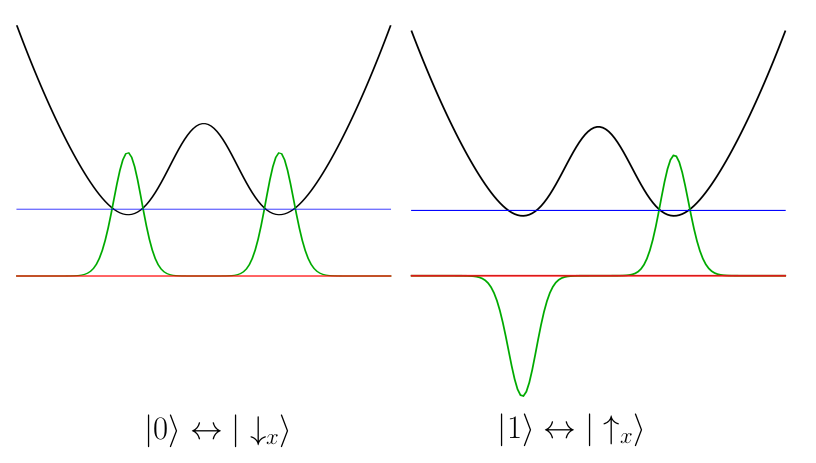
\includegraphics[width=0.7\textwidth]{Figures/eigen_functions.png}

\caption{First eigenfunctions of a double well potential}
\label{fig:double_well_eigen}
\end{figure}

These two eigen-functions can be combined by addition and subtraction to create combinations of even and odd parity as 
\begin{equation}
\ket{L}=\frac{1}{\sqrt{2}}(\ket{0}-\ket{1})\qquad,\qquad \ket{R}=\frac{1}{\sqrt{2}}(\ket{0}+\ket{1}).
\end{equation}
The resulting wave functions of these operations are shown in Figure \ref{fig:double_well_eigen_sum}. These eigenfunctions then represent in the language of wave functions a particle located on the left or the right side of the double well potential as a discrete two level system, this reinforces the idea of using the continuous variable subject to the double well potential to validate the model we will be using.

\begin{figure}[H]
\centering
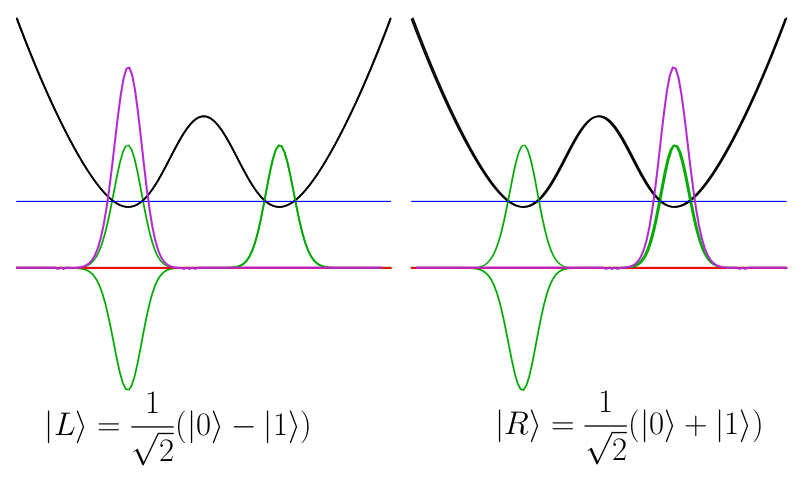
\includegraphics[width=0.7\textwidth]{Figures/eigen_functions_sum.png}

\caption{Sum of the eigen-functions of a double well potential}
\label{fig:double_well_eigen_sum}


\end{figure}



\subsection{Heat bath proper modeling}

The system described in the last subsection can be described by the hamiltonian given by

\begin{equation}
H=-\frac{1}{2}\hbar\Delta_0\sigma_x	+\frac{1}{2}\epsilon\sigma_z,
\end{equation}
where $\hbar\Delta_0$ is the tunneling matrix between the two wells, $\epsilon$ is a detuning parameter between the ground states of the two wells and $\sigma_i(i=x,y,z)$ are the Pauli matrices. When this hamiltonian is completely isolated then the problem can be solved exactly, different happens when it is not isolated. In real life, any two level system is continuously interacting with an environment so it becomes a necessity to model an environment properly in order to understand in a more detailed degree the dynamics the two level system may have. Generally in open quantum systems literature \cite{leggett1987dynamics} the way the interaction of an environment with the central system is modeled is by coupling the system with an environment  of the form $\sigma_z\hat{\Omega}$ where $\hat{\Omega}$ is an operator of the environment. When the coupling is considered in this way will let the environment to be sensitive to the state $\sigma_z$ of the system, this way we can say that the environment can help as an observer of the central system by interacting with the state $\sigma_z$. If the environment is taken as a bosonic heat bath then this approach leads to the commonly known \say{spin-boson} hamiltonian with a given spectral function $J(\omega)$.


\section{Dynamics of the system}
In this section we will describe the mathematical properties of the system as a classical hamiltonian problem. We will study the different dynamics the system will have as afunction of its parameters, we will treat the heat bath as a finite heat bath instead of the common infinite heatbath in the microscopic theory of dissipation in Langevin dynamics. We will evidence here that even if the heat bath is not infinite, it will mimic the dissipation of an infinite heat bath.

\subsection{Hamilton equations of motion}
The model of a particle coupled to a heat bath that we will study here is described by the following hamiltonian:
\begin{equation}
H(p,x;\textbf{P,X})=H_{S}+H_B+H_{SB}
\label{eq:total_hamiltonian}
\end{equation}

Where the hamiltonian for the central system $(S)$ can be viewed as a particle of mass $m$ moving in a double well potential of quartic nature. The corresponding hamiltonian reads as
\begin{equation}
H_{S}=\frac{p^2}{2m}-a\frac{x^2}{2}+b\frac{x^4}{4},
\label{eq:particle_hamiltonian}
\end{equation}

where $p$ is the momentum of the particle, $q$ is te position of the particle, and $a,b$ are parameters that change the shape of the potential.The hamiltonian for the bath $(B)$ is described as a set of harmonic oscillators
\begin{equation}
H_B(\textbf{P,X})= \sum_{n=1}^N \Big(\frac{P_n^2}{2M_n}+M_n \omega_n^2\frac{X_n^2}{2} \Big),
\label{eq:bath_hamiltonian}
\end{equation}

each oscillator $n$ posses position $X_n$, momentum $P_N$, frequency $\omega_n$ and mass $M_n$. The last term of the hamiltonian consists on the interaction term where the system and bath positions are coupled bilinearly according to
\begin{equation}
H_{SB}(p,x;\textbf{P,X})=-x\sum_{n=1}^N g_n X_n+x^2 \sum_{n=1}^N\frac{g_n^2}{2M_n \omega_n}
\label{eq:interaction_hamiltonian}
\end{equation}
The last term here acts as a counter term whose job is to renormalize the potential when the interaction between the oscillators is present. This hamiltonian is often called the Caldeira-Leggett hamiltonian \cite{caldeira1981influence}.\par 

The hamilton equations for this hamiltonian can be separated in the two parts, the particle and the heat bath. The hamilton equations of the particle read as

\begin{equation}
\dot{p}=\frac{-\partial H}{\partial x}=ax-bx^3+\sum_{n=1}^N g_n X_n-x\sum_{n=1}^N \frac{g_n^2}{M_n \omega_n^2},
\end{equation}

\begin{equation}
\dot{x}=\frac{\partial H}{\partial p}=\frac{p}{m}.
\end{equation}

For the heat bath we find that the equations of motion for each of the $n$ oscillators are given by
\begin{equation}
\dot{P_n}=\frac{-\partial H}{\partial X_n}=-xg_n-M_n \omega _n ^2 X_n
\end{equation}

\begin{equation}
\dot{X_n}=\frac{\partial H}{\partial P_n}=\frac{P_n}{M_n}
\end{equation}

From these equations we can calculate the frequency of small oscillations for the double well potential, we proceed by taking the the potential given as
\begin{equation}
V(x)=-\frac{1}{2}ax^2+\frac{1}{4}bx^4,
\label{eq:potential}
\end{equation}
the equilibrium points are located where the potential $V$ is minimum or maximum, this is when the following condition is satisfied
\begin{equation}
\frac{d}{dx}V=0\rightarrow x(bx^2-a) = 0.
\end{equation}

The solutions for this equation are $x=0,\pm \sqrt{\frac{a}{b}}$, where $x=0$ is an unstable equilibrium point and $x=\pm \sqrt{\frac{a}{b}}$ are stable equilibrium points \par 
We proceed to perform a Taylor expansion around a stable equilibrium point say $x_0=\sqrt{\frac{a}{b}}$ as
\begin{equation}
V(x_0 +\epsilon )=V(x_0)+U'(x_0)\epsilon + \frac{1}{2}V''(x_0)\epsilon ^2 + ...
\end{equation}
The first term on the right side is a constant term, this means it can be ignored. The second term is equal to zero due to the fact that $V'(x_0)=0$ is the condition for the stable minimum. The third term will be according to the result of $V''(x_0)=\frac{1}{2}(-a+3bx^2)| _{x=x_0}$, this results in the following expansion
\begin{equation}
V(x_0+\epsilon)\approx \frac{1}{2}(2a)\epsilon ^2.
\end{equation}
This potential is the same expression of a harmonic oscillator potential with a spring constant of $k=2a$ (compared with the harmonic oscillator potential $V_{HO}=\frac{1}{2}kx^2$). This means that the frequency of small oscillations around the stable minimum is given by

\begin{equation}
\omega =\sqrt{\frac{k}{m}}=\sqrt{\frac{2a}{m}}
\label{eq:freq_small_oscillations}
\end{equation}

For the case of the particle coupled to the heat bath we can do the same analysis and see the role of the counter term in the hamiltonian resulting in the same results as above. The equilibrium points of the whole hamiltonian must satisfy the following condition

\begin{equation}
\frac{d}{d\textbf{x}}H=0\rightarrow \frac{d}{dx}H =0 \quad , \quad \frac{d}{dX_n}H  = 0.
\end{equation}
Evaluating the derivatives we arrive to the following equations
\begin{equation}
x(bx^2-a)-\sum_{n=1}^N g_n X_n +\sum_{n=1}^N \frac{xg_n^2}{M_n\omega_n}=0 \quad , \quad xg_n=M_n\omega_n^2 X_n 
\end{equation}
where the right hand side equation will provide the constraint to retrieve the original conditions of equilibrium for the potential on the right hand side
\begin{equation}
x(bx^2-a)-\sum_{n=1}^N g_n X_n +\sum_{n=1}^N \frac{xg_n^2}{M_n\omega_n}= x(bx^2-a)-\sum_{n=1}^N g_n X_n +\sum_{n=1}^N g_n X_n=x(bx^2-a)=0.
\end{equation}
We can also calculate the height of the potential barrier (the difference between the height of the unstable equilibrium with the stable equilibrium), we can do this by insterting one of the minima on equation (\ref{eq:potential}):
\begin{equation}
V(\sqrt{\frac{a}{b}})=-a\frac{a}{2b}+b\frac{a^2}{4b^2}=\frac{-a^2}{2b}+\frac{a^2}{4b}=-\frac{a^2}{4b},
\end{equation}
For this particular situation the unstable equilibrium is located at the $0$ height, meaning that in general the height of the potential barrier will be the difference between the unstable and the equilibrium point given as
\begin{equation}
PB(a,b)=\frac{a^2}{4b}
\label{eq:PB_eq}
\end{equation}



\subsection{Infinite heat bath and dissipation}
In the limit of infinite oscillators, the system approaches to irreversible dynamics such as in the case of a system with dissipation. In the case of our hamiltonian (\ref{eq:total_hamiltonian}) where we are interested in a linear coupling of the oscillator with the central system (\ref{eq:interaction_hamiltonian}) the dissipation takes the form of a damping term proportional to the velocity of the central system such as in the case of a harmonic oscillator in a viscous fluid. This damped dynamics will then have the Newton equation of motion given as:
\begin{equation}
m\ddot{x}+\lambda x\dot{x}-ax+bx^3=0,
\label{eq:newton_damped}
\end{equation}
this equation is identical to the unforced version of the Duffing oscillator \cite{guckenheimer2013nonlinear}, where $\lambda$  is the damping coefficient that will be defined by the nature of the coupling coefficient $g_0$ of the heat bath.

\begin{figure}[H]%
    \centering
    \subfloat[Changing only $b$]{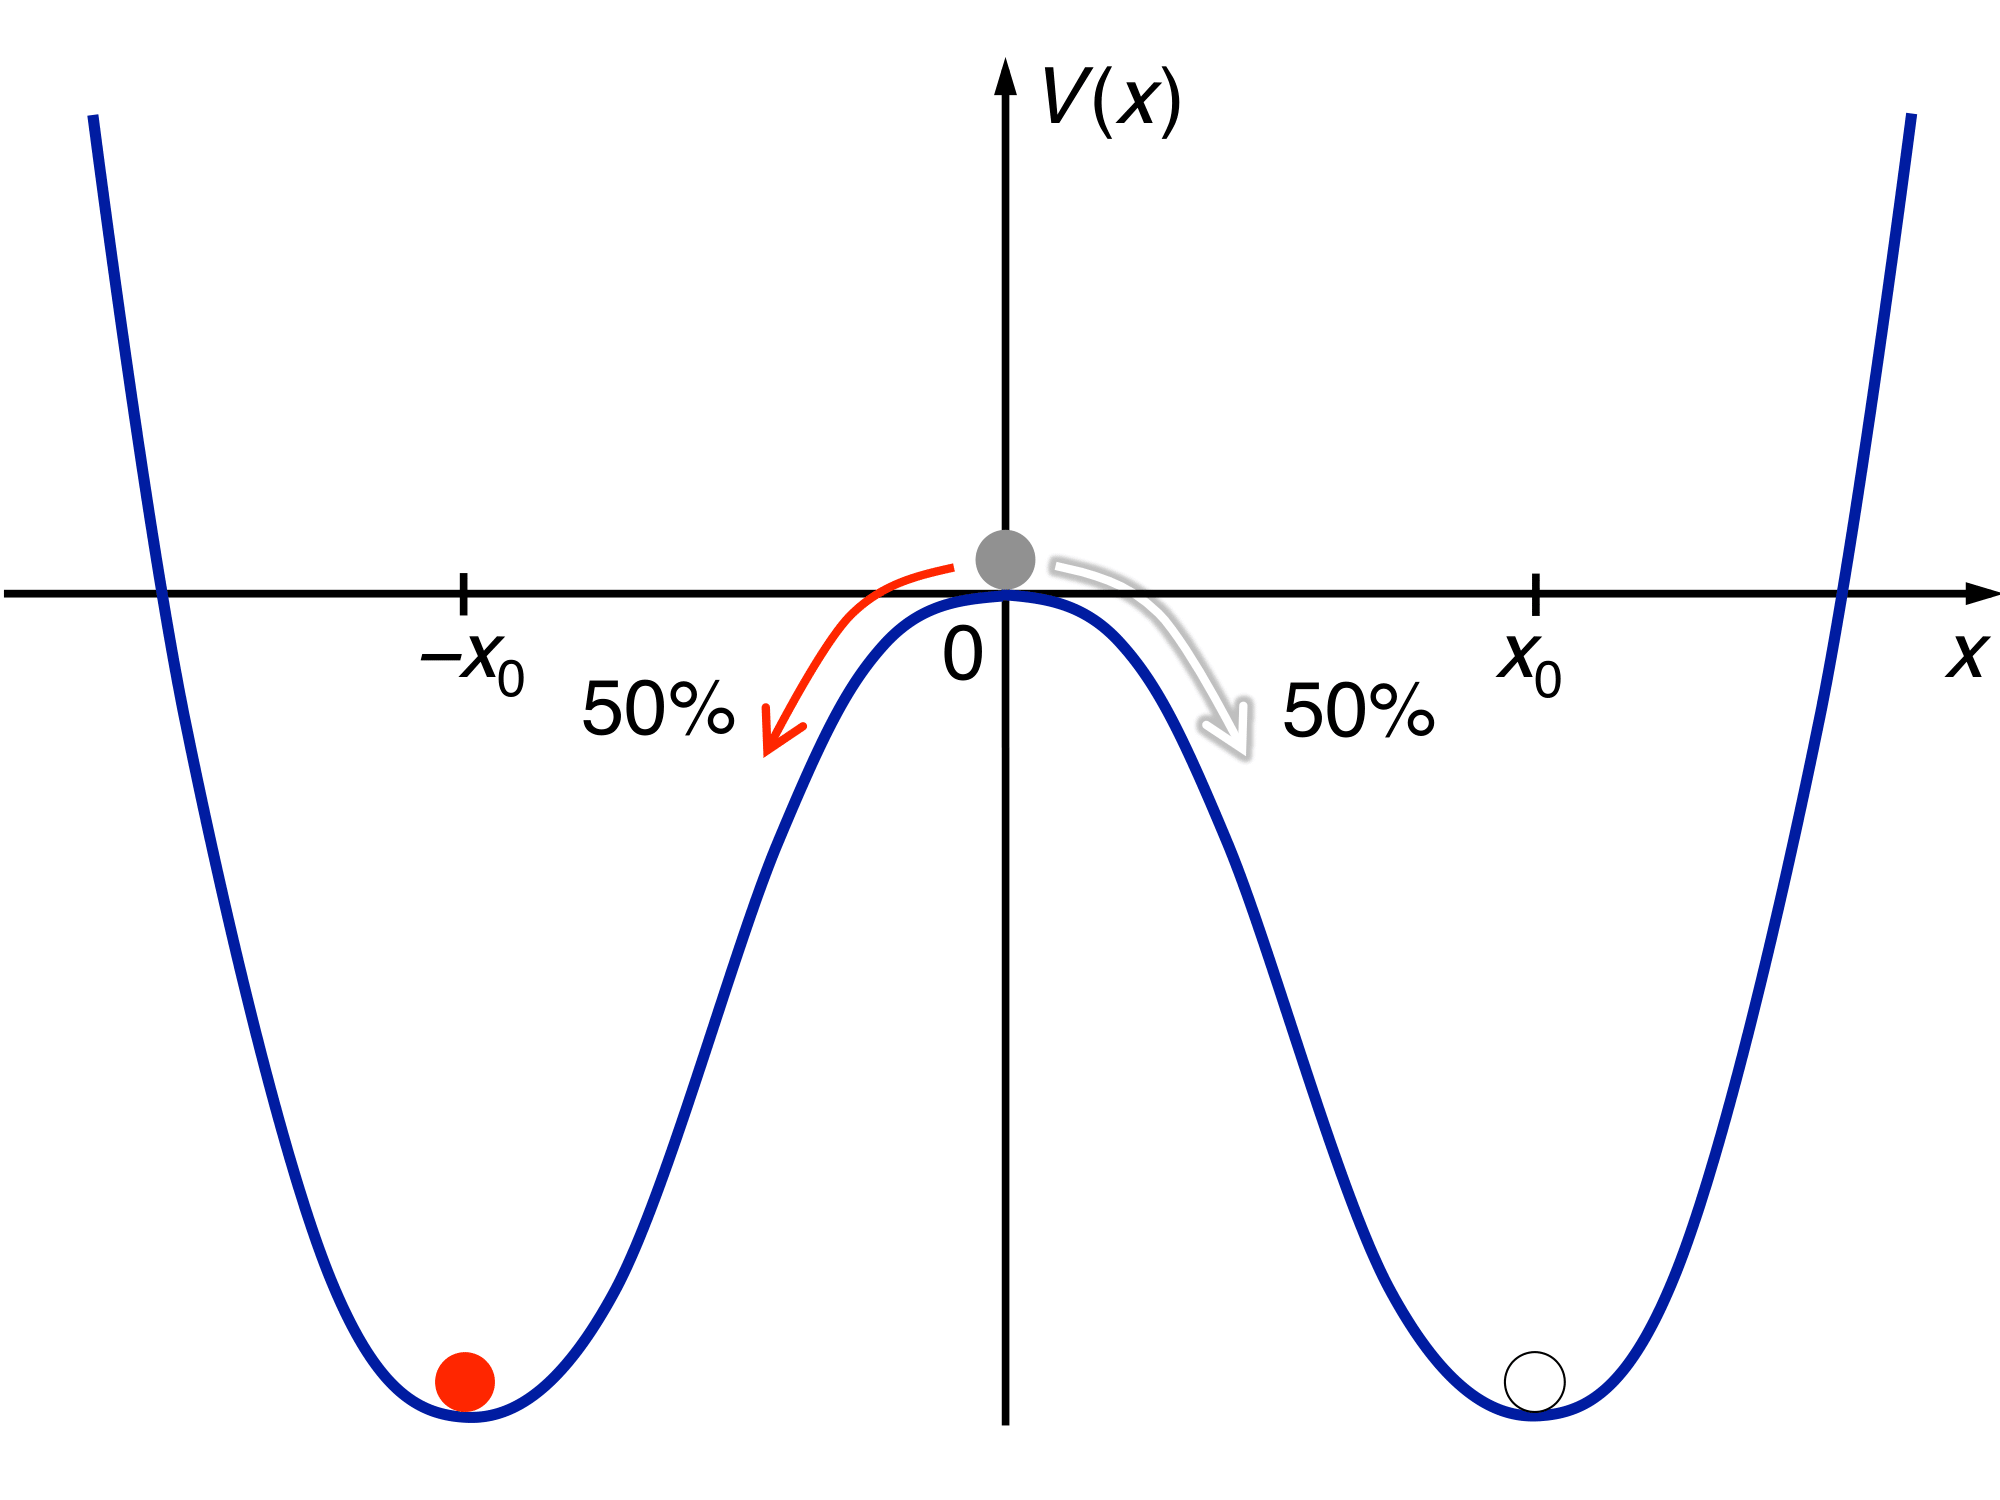
\includegraphics[width=7cm]{Figures/doublewella.png} }%
    \qquad
    \subfloat[Changing $a$ and $b$ but keeping the ratio $a/b=2$]{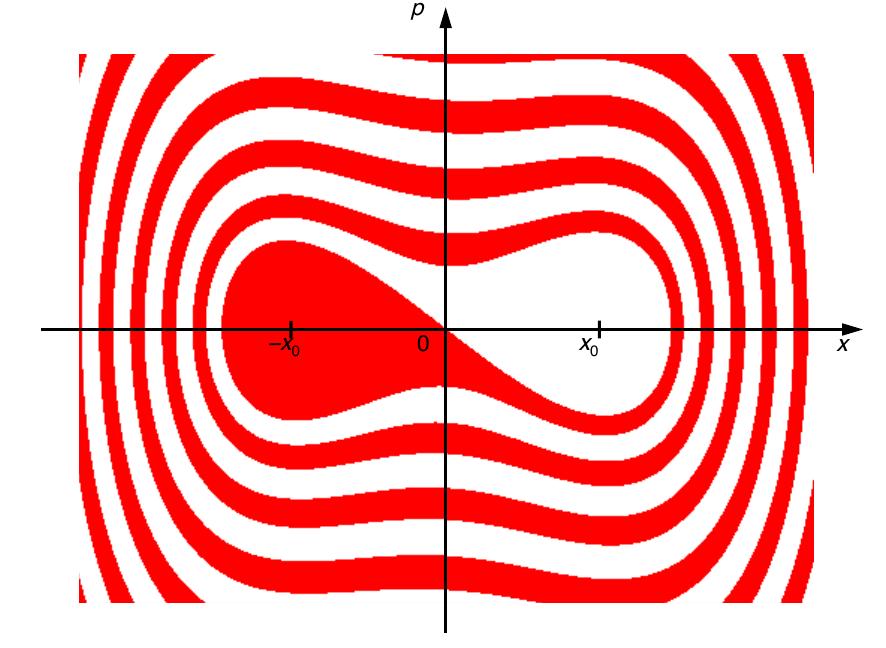
\includegraphics[width=7cm]{Figures/doublewell-1.png} }%
    \caption{Number of jumps between the wells as a function of the number of oscillators in the heat bath for different values for the height of the potential barrier $PB$}%
    \label{fig:changing_PB}%
\end{figure}


\subsection{Poincaré surface plots for finite heat bath}
We start the numerical experiments of this model with only one oscillator coupled to the particle of the central system. This very simple model already exhibits the traits and characteristics of a chaotic system, this is due to the barrier of the unstable equilibrium position. We can illustrate this by picturing the particle moving on the double well potential without any coupling with the heat bath, if the particle has enough energy, it will move freely between the two wells, otherwise it will orbit around one well. This can be seen in two different ways, the first one is by looking at the potential part of the hamiltonian of each part of the whole system i.e. the quartic potential and the harmonic oscillator potential, plotting each potential along an axis we can see the contours of energy for the dynamics of the system.

\begin{figure}[H]
\centering
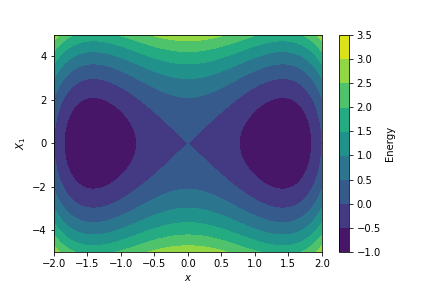
\includegraphics[width=0.7\textwidth]{Figures/energy_contour.png}
\caption{Energy contour of the double well potential on the $x$ axis and the harmonic oscillator potential on the $y$ axis for $m=1$, $a=2$, $b=1$, $\omega_1=1.5$, $M_1=0.1$ and $g_1=0$}
\label{fig:contour_g0}
\end{figure}

In Figure (\ref{fig:contour_g0}) we see that as the dynamics is uncoupled, the particle moves freely on the double well potential and the harmonic oscillator doesn't really changes its motion. \par 

Following this representation we can observe the perturbation induced by the harmonic oscillator when we \say{turn on} the coupling between the two systems, for a coupling of $g_1=0.1$ it is already evident that shape of the whole potential suffers a shearing effect:

\begin{figure}[H]
\centering
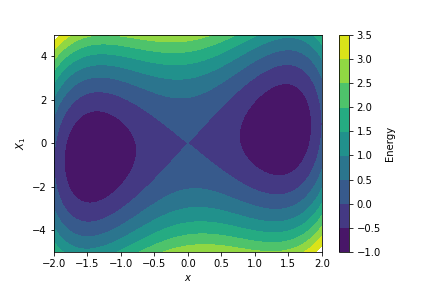
\includegraphics[width=0.7\textwidth]{Figures/energy_contour_coupled01.png}
\caption{Energy contour of the double well potential on the $x$ axis and the harmonic oscillator potential on the $y$ axis for $m=1$, $a=2$, $b=1$, $\omega_1=1.5$, $M_1=0.1$ and $g_1=0.1$\label{fig:contour_g01}}

\end{figure}
This means that independently of the initial conditions of the particle, the motion will be certainly affected by the presence of the potential due to the harmonic oscillator.\par 

Now that we have seen a visual representation of the system without solving the equations of motion of the system, it is necessary to take a look at the specific dynamics of the system numerically by using a symplectic integrator. The integrator of our choice is the Calvo Sanz-Serna 4th order symplectic integrator \cite{gray1994symplectic}\cite{sanz1993symplectic}\cite{rackauckas2017differentialequations}, we use a timestep defined by $dt=0.05*T$ where $T=\frac{2\pi}{\omega_t}$ is the period of a harmonic oscillator of frequency $\omega_t=12$. Here we set up different initial conditions for the particle along its phase space, the position of the oscillator always to start at $X_1=0$ and fixed the energy (twice the energy of the potential barrier between the wells here) as a constraint to be followed by the initial momentum of the oscillator. Each point of the Poincaré section is registered as the event when the oscillator crosses its equilibrium position $X_1=0$ with a possitive momentum. We will take a number of initial conditions along the phase space of the particle and start to increase the coupling to see the behavior of the orbits in the phase space of the particle.

\begin{figure}[H]
\centering
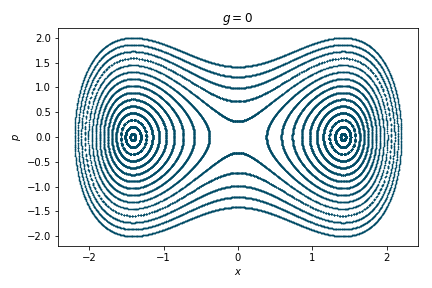
\includegraphics[width=0.7\textwidth]{Figures/poincare_g0.png}
\caption{Poincaré surface plot for the particle phase space for $m=1$, $a=2$, $b=1$, $\omega_1=1.5$, $M_1=0.1$ and $g_1=0$
}
\label{fig:poinc_g0}
\end{figure}

In Figure (\ref{fig:poinc_g0}) we start with $g_1=0$ and see that the orbits on the phase space of the particle are closed, the particle is totally unaware of the harmonic oscillator's potential. Now we will slowly start to \say{turn on} the coupling between the systems.\par 


\begin{figure}[H]
\centering
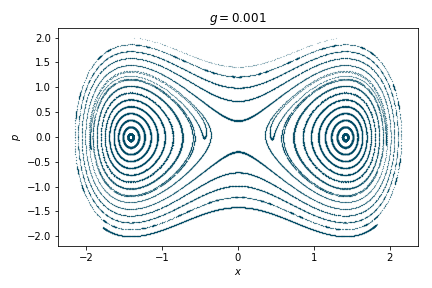
\includegraphics[width=0.7\textwidth]{Figures/poincare_g0001.png}
\caption{Poincaré surface plot for the particle phase space for $m=1$, $a=2$, $b=1$, $\omega_1=1.5$, $M_1=0.1$ and $g_1=0.001$
}
\label{fig:poinc_g0001}
\end{figure}

As soon as there is coupling present in the dynamics of the system the orbits start to destroy progresively as we can see in this Figure (\ref{fig:poinc_g0001}). 

\begin{figure}[H]
\centering
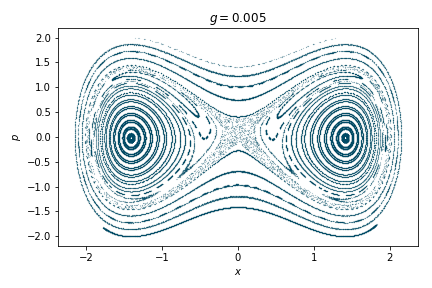
\includegraphics[width=0.7\textwidth]{Figures/poincare_g0005.png}
\caption{Poincaré surface plot for the particle phase space for $m=1$, $a=2$, $b=1$, $\omega_1=1.5$, $M_1=0.1$ and $g_1=0.005$
}
\label{fig:poinc_g0005}
\end{figure}

The section of phase space where we start to see pure chaos at first is when the energy of the particle is very close to the energy of the barrier between the two wells as we can see in Figure (\ref{fig:poinc_g0005}), this particular behavior around this points is of particular interest for our case as we will later use the unstable equilibrium position as the initial condition for the particle.

\begin{figure}[H]
\centering
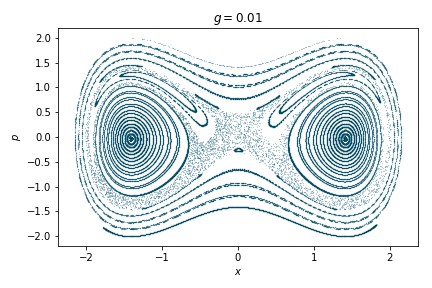
\includegraphics[width=0.7\textwidth]{Figures/poincare_g001.png}
\caption{Poincaré surface plot for the particle phase space for $m=1$, $a=2$, $b=1$, $\omega_1=1.5$, $M_1=0.1$ and $g_1=0.01$
}
\label{fig:poinc_g001}
\end{figure}
As we continue to increase the coupling strength we progress on the destruction of the orbits and approach to a more chaotic behavior.

\begin{figure}[H]
\centering
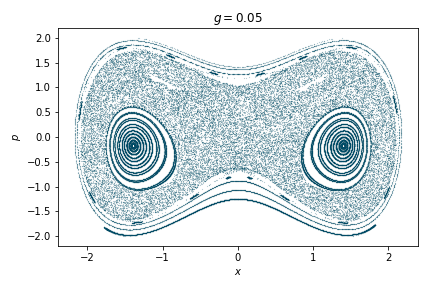
\includegraphics[width=0.7\textwidth]{Figures/poincare_g005.png}
\caption{Poincaré surface plot for the particle phase space for $m=1$, $a=2$, $b=1$, $\omega_1=1.5$, $M_1=0.1$ and $g_1=0.05$
}
\label{fig:poinc_g005}
\end{figure}

\begin{figure}[H]
\centering
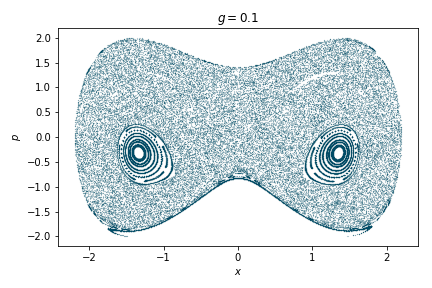
\includegraphics[width=0.7\textwidth]{Figures/poincare_g01.png}
\caption{Poincaré surface plot for the particle phase space for $m=1$, $a=2$, $b=1$, $\omega_1=1.5$, $M_1=0.1$ and $g_1=0.1$
}
\label{fig:poinc_g01}
\end{figure}
Finally in Figure (\ref{fig:poinc_g01}) we arrive to the coupling we used for Figure (\ref{fig:contour_g01}) $g=0.1$. As we can see from the poincaré section, the overall behavior of the system is very chaotic except for the stable islands very near to the condition of the particle to have small energy located near to the stable equilibrium points  with a small momentum. Comparing these two pictures we can see that even if the shearing behavior observed in the contour plots can barely be noticed, the dynamics of the system is almost completely chaotic.\par 

Just for illustration we calculated the poincare section for $g=0.2$ to show that the behavior of pure chaos continues to increase, this is shown in Figure (\ref{fig:poinc_g02}).

\begin{figure}[H]
\centering
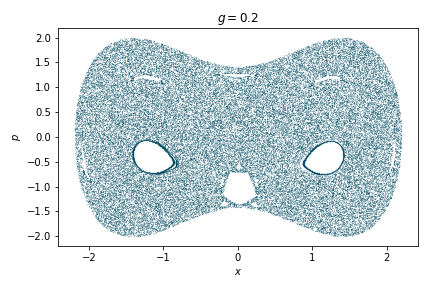
\includegraphics[width=0.7\textwidth]{Figures/poincare_g02.png}
\caption{Poincaré surface plot for the particle phase space for $m=1$, $a=2$, $b=1$, $\omega_1=1.5$, $M_1=0.1$ and $g_1=0.2$
}
\label{fig:poinc_g02}
\end{figure} 


\subsection{Dynamics for 1 oscillator}
We have seen in the previous subsection that with only one oscillator, the system is immediately chaotic. We will now study the usual trajectories that the central system will follow for only one oscillator. The conditions for the general parameters of these cases will be similar to the ones of the previous section. 

\begin{figure}[H]
\centering
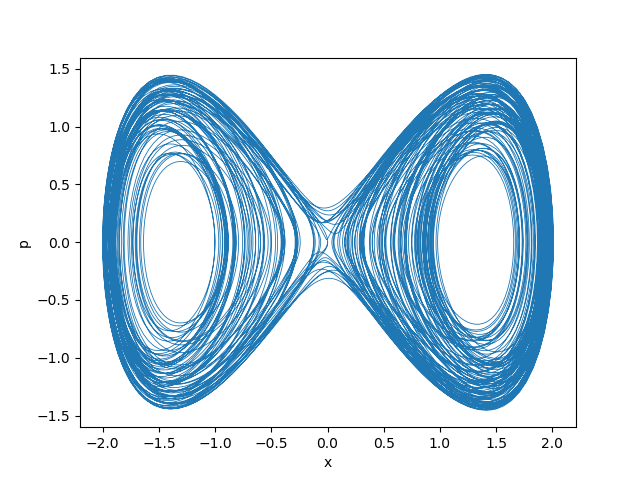
\includegraphics[width=0.7\textwidth]{Figures/one_osci_tray.png}
\caption{Typical trajectory in phase space of the particle in the double well potential coupled to one oscillator
}
\label{fig:one_osci_tray}
\end{figure} 

 In Figura (\ref{fig:one_osci_tray}) we see a typical trajectory of the particle interacting with a harmonic oscillator, we see that the particle falls to one well and the other in an erratically way. The chaotic dynamics makes it difficult to predict to which side the particle will fall when the dynamics begins. The phase space trajectory permits the
 
\begin{figure}[H]
\centering
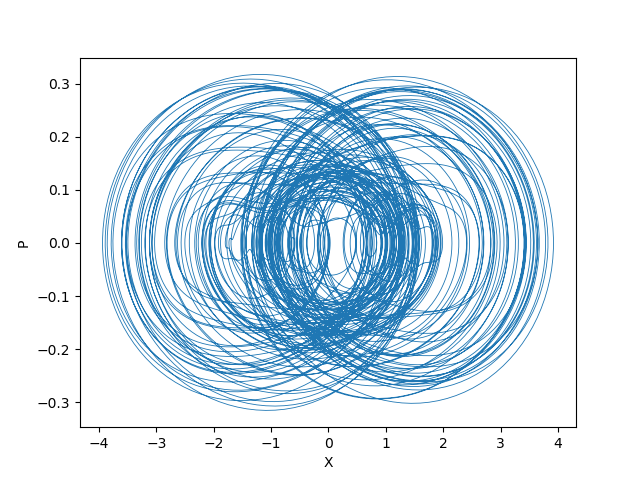
\includegraphics[width=0.7\textwidth]{Figures/one_osci_tray_osci.png}
\caption{Typical trajectory in phase space of the oscillator coupled to the particle in the double well potential 
}
\label{fig:one_osci_tray_osci}
\end{figure} 

In Figure (\ref{fig:one_osci_tray_osci}) we can see the phase space trajectory of the harmonic oscillator and how it is perturbed compared with a typical trajectory of  a harmonic oscillator without a coupling whose orbits in phase space are perfect ellipses. it is to note that the dynamics is antisymmetric with the inversion of the initial conditions of the harmonic oscillator $X_1\rightarrow -X_1$ and $P_1 \rightarrow -P_1$ will lead to the particle falling into the opposite well.


\subsection{Dynamics for 2 oscillators}
When we start to increase the number of harmonic oscillators that compose the heat bath we start to evidence the tendency to stay on one well for a longer period of time as it is shown in Figure (\ref{fig:two_osci_tray}) .

\begin{figure}[H]
\centering
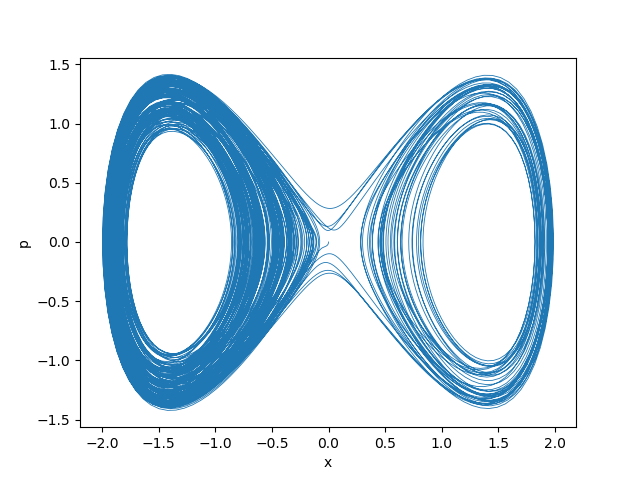
\includegraphics[width=0.7\textwidth]{Figures/two_osci_tray.png}
\caption{Typical trajectory in phase space of the particle in the double well potential coupled to two oscillator 
}
\label{fig:two_osci_tray}
\end{figure} 

The harmonic oscillators will share some of the initial energy of the particle for a longer time and  this means that the particle will take longer to have again enough energy to jump from one well to the other. 



\section{Nature of the heat bath}
It is natural to consider the possibilities in this particular problem were we can vary a big amount of parameters to search for different dynamics and properties that exhibit the system, the model is rich in quantities that can be calculated and extracted from it. This idea also plays against our odds because as there are many parameters to play with it is difficult to control the whole system in an optimal and hierarchical way. There are two types of parameters that we will monitor very closely: the frequency spectra and the energy spectra for the heat bath; these two parameters contain the information regarding the nature of the heat bath, meaning we can model different behaviors of the heat bath interacting with the particle. In this section we will give a little insight on the importance of correctly modeling the nature of the heat bath.


\begin{figure}[H]
\centering
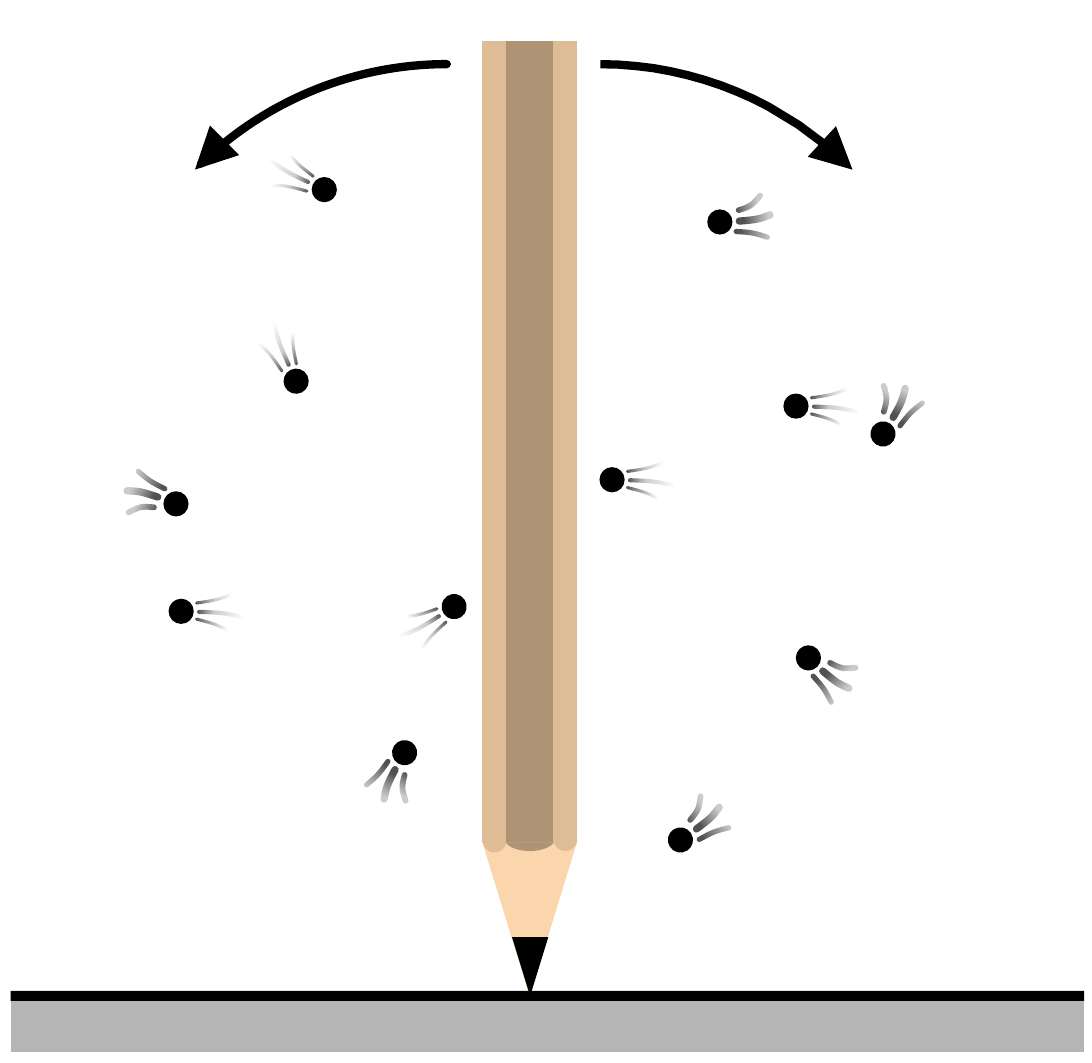
\includegraphics[width=0.4\textwidth]{Figures/pencilonend-1.png}
\caption{Pencil immersed in an environment that we can consider as a heat bath.
}
\label{fig:pencil}
\end{figure}

The importance to model correctly the heat bath is related to the idea of this numerical experiment. We shall imagine this problem as a pencil perfectly balanced on its tip, it is of course an unstable equilibrium point, therefore the slightest perturbation of this pencil will cause the pencil to fall somewhere, if we imagine this on a two dimensional plane, the pencil will either fall left or right. Then modeling the bath in a correct numerical way will give us the way these perturbations considered as an environment will affect the state of the initially balanced pencil. This environment may have different parameters to vary in order to have different dynamics for the pencil.\par 

In principle we can consider the whole system of particle$+$bath as a compound closed system, but if we look at just the particle in the double well then it can be considered as an open system interacting with its environment given by the heat bath. When the number of oscillators in the heat bath is small, then the poincaré recurrence time will be also small as the particle will exchange energy with the heat bath in a short period of time. Nevertheless when the number of harmonic oscillators increases then the poincaré recurrence time will increase also, in the limit of infinite harmonic oscillators the poincaré recurrence time will also go to infinity producing dissipation phenomena in the system\cite{mazur1960poincare}.


\subsection{Frequency spectra}
The way the frequencies of the harmonic oscillators are distributed in this work is taken from the theory of quantum dissipation in open systems.  When the system is composed by a huge number of harmonic oscillators it is convenient to choose wisely how the frequencies of harmonic oscillators are distributed, therefore we may introduce the idea of the spectral density of bath modes as
\begin{equation}
J(\omega) =\pi \sum_{i=1}^N\frac{g_i^2}{2_i\omega_i}\delta (\omega-\omega_i).
\end{equation}
This quantity will in fact give the information about how the heat bath's frequencies relate and include how the coupling to the system is chosen characterizing the bath. Depending on the system to be studied different values for the parameters may be taken to reproduce different dynamics, in the case of infinite modes this spectral density will relate to the damping integral kernel characterizing the Langevin dissipative dynamics.\par 
In this work we will take the distribution of the frequencies as in standard open systems dynamics\cite{leggett1987dynamics} \cite{wang2010coherent}\cite{wang2008coherent}

\begin{equation}
J(\omega) \sim w^s f(\omega,\omega_c)
\label{eq:spectral_density}
\end{equation}
Where $\omega_c$ is the characteristic frequency of the bath, and $f(\omega,\omega_c)$ is a damping function which helps $J(\omega)$ to vanish in the limit of $\omega \rightarrow \infty$. There are many different ways to choose $f(\omega,\omega_c)$ \cite{wang2008coherent}, in this case we will choose an exponential cut-off damping type as $f(\omega,\omega_c)=e^{-\omega/\omega_c}$.   

\begin{figure}[H]
\centering
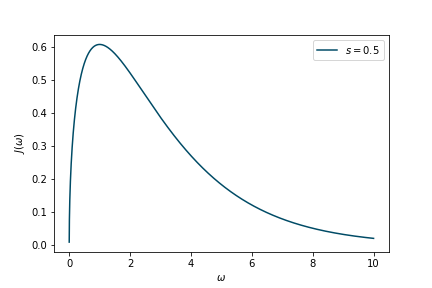
\includegraphics[width=0.7\textwidth]{Figures/frequency_spectra.png}
\caption{Frequency spectrum distribution without normalization for the case of $s=0.5$.
}
\label{fig:frequency_spectra}
\end{figure} 


\subsection{Energy spectra}
In this work we will monitor the energy spectra in two different ways, both are related to the idea of having a cloud of harmonic oscillators with initial conditions around the origin of phase space. The first idea is by  drawing the energy of the oscillators from a distribution with a certain mean and variance, the second one consists of using the Box-Muller transform to sample a quasi-gaussian two dimensional distribution of harmonic oscillators in phase space.  Essentially both of these cases will relate to a gaussian distribution in energies of the heat bath, we will model most of the times a cold heat bath i.e. with small energy compared to the central system, therefore it the energy distribution does not need to be necessarily a Boltzmann distribution.
\subsubsection{Drawing energy from a distribution}
The method outlined in this subsection consists on drawing the energy of each harmonic oscillator from a probability distribution (mostly a gaussian) with a determined mean and variance. This method will let us normalize the energy of the heat bath at will, having the energy of each harmonic oscillator will let us compute the sum and divide each energy by the normalization desired.\par 
Now to decide where to locate each oscillator we sample a random number from a uniform distribution $[0,2\pi)$, this will represent an angle on a circle which will be deformed into an ellipse according to the energy and frequency of each harmonic oscillator obtaining finally a position of a harmonic oscillator according to a determined energy ellipse. This process is repeated for every oscillator on the bath giving as a result a distribution of oscillators in phase space with an energy distribution of the heat bath perfectly defined and normalized.

\subsubsection{Quasi-gaussian distribution in phase space}
This method consists in implementing the Box-Muller transform algorithm onto a uniform distribution to obtain a two dimensional distribution grid of points that represent a gaussian with a defined mean and variance along each dimension \cite{box1958note}. This method is important in the way that it allows us to have a gaussian distribution in phase space for the harmonic oscillators that can be canged at will to have a defined width along position or momentum as desired, this feedom in choosing the shape of the distribution gives us freedom in the nature of the heat bath on how the harmonic oscillators' motion changes in the initial conditions have different consequences in the particle's motion. This method can also be normalized efficiently.





\section{Number of modes in the bath}
A very important parameter to determine the dynamics of the system is the number of oscillators in the heat bath. According to dissipative dynamics theory, we retrieve an equation of Langevin type dynamics in the limit of infinite harmonic oscillators in the bath.We have already shown the behavior of the dynamics under the influence of only one harmonic oscillator coupled to the particle. What we will do in this work will be increase steadily the number of harmonic oscillators of a finite heat bath to achieve dissipative behavior without the need of extending the system to infinity. Therefore, it is important to keep an eye on the dynamics of each case of the number of harmonic oscillators and change different parameters of the system in order to understand in a more general way the behavior of the whole system as a function of the number of modes of the bath. This analysis will lead to the conclusion to modelate dissipative dynamics in a finite heath bath with a very small number of modes.

\subsection{Chaos to dissipative dynamics}
In this section we will start to evidence the loss of chaotic dynamics due to the increasing number of oscillators. 


\subsection{Variation of the double well and heat bath parameters}
There are four types of parameters that are interesting for us to look at the variation of the dynamics of the system: The exponent $s$ in the  equation (\ref{eq:spectral_density}), the coupling constant of the oscillators $g_0$ that multiplies the coupling constant of each oscillator $g_i=g_0/\sqrt{N}$, the height of the potential barrier and the initial energy of the heat bath. Each of these conditions will affect the number of jumps from one well to the other that the particle makes. We will therefore evaluate the results of changing these parameters for different number of oscillators for $100$ test cases where the positions, frequencies and energies are randomized every time and the numbers of jumps will be averaged. The way of sampling the energies and initial conditions are described in the method of drawing energies from a gaussian distribution in order to have more control on the energies of the harmonic oscillators. For most of the cases we will use fixed values for each parameter unless explicitly stated otherwise, these values are $s=0.5$, $g_0=0.1$, the initial energy of the heat bath $E_{bath}=0.1$ and the height of the potential barrier $PB=1$

\subsubsection{Changing the exponent $s$}
According to the microscopic theory of dissipation \cite{leggett1987dynamics}, the exponent $s$ in equation (\ref{eq:spectral_density}) controls the nature of the bath where $s=1$ is the \say{ohmic} case where it can be compared to a dissipative term proportional to velocity in the classical equation. The case of $s>1$ is called \say{super-ohmic} and the case of $0<s<1$ is called \say{sub-ohmic}. Here we observe the behavior of the system in terms of the jumps between the wells seen for different numbers of harmonic oscillators and different values of the parameter $s$. \par

\begin{figure}[H]
\centering
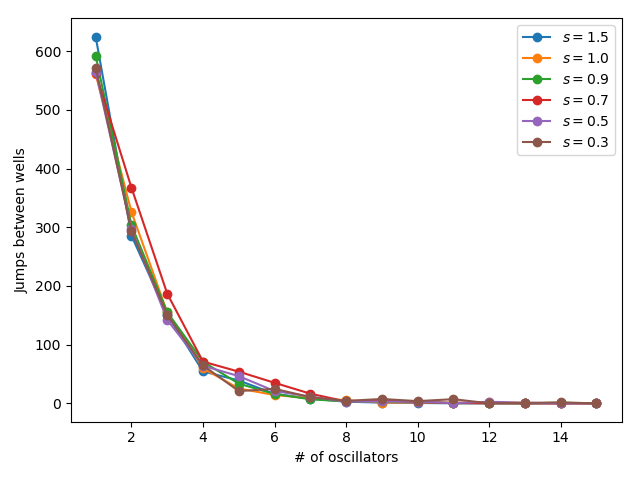
\includegraphics[width=0.7\textwidth]{Figures/change_s_number.png}
\caption{Number of jumps between the wells as a function of the number of oscillators in the heat bath for different values of the parameter $s$ of the spectral function.
}
\label{fig:changing_s}
\end{figure} 

We conclude that for the classical case, the parameter $s$ in the spectral density does not really affect the dynamics of the system in a particular way as we don't see a real difference between having a bath with sub-ohmic, ohmic or super-ohmic nature. We see the general behavior of dissipation where the jumps between the wells decrease with the increase in the in the number of oscillators in the heat bath and it is independent of the parameter $s$.

\subsubsection{Changing the individual coupling $g_0$}
We have seen the effect of the coupling involving chaos with only one oscillator in one of the previous sections, this showed us the effect of different values for the coupling constants that develop into increasing chaotic motion. In this section we will continue to study the effects on the dynamics of the whole system when we use different values for the constant $g_0$ that multiplies each of the individual coupling constants $g_i \sim 1/\sqrt{N}$. Previously, the method we used to describe the dynamics and the effects of the change in the coupling was the Poincaré surface section, with this method we could visualize the increase of chaotic dynamics when the rational tori got destroyed. Unfortunately, when we increase the number of harmonic oscillators, the Poincaré sections stop being very useful, this is due to the amount of degrees of freedom the system will have. We could visualize the dynamics of the system because there was only two degrees of freedom, this made it possible to find planes where the dynamics was projected and this were the Poincaré surface sections, when we increase the number of oscillators the Poincaré planes will become hyperplanes that we cannot visualize properly, this means we would have to project the planes onto lower dimensions but doing this we would loose most of the details of the dynamics. For this reason we will visualize the change of the behavior using the same method of analysing the frequency of jumps between the wells.\par 

We simulated the dynamics of the $100$ test cases for different values of $g_0$ and different number of harmonic oscillators. We know from previous the experience of only one oscillator that if the coupling is strong the overall behavior will tend to be more chaotic, but now that we have more harmonic oscillators we start to see the effects of dissipation over chaos. A big coupling constant will continue to result in strong interactions between the oscillators and the particles, but the tendency of the particle to stay on one side will prevail.

\begin{figure}[H]
\centering
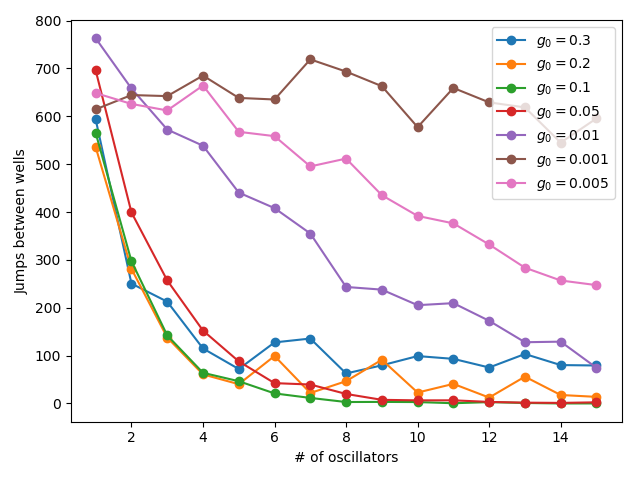
\includegraphics[width=0.7\textwidth]{Figures/change_g_number.png}
\caption{Number of jumps between the wells as a function of the number of oscillators in the heat bath for different values of the coupling constant  $g_0$ of each oscillator.
}
\label{fig:changing_g}
\end{figure} 

In Figure (\ref{fig:changing_g}) we evidence that the overall tendency of dissipation is observed when the number of harmonic oscillators increases regardless the coupling constant $g_0$ (for $g=0.001$ in the figure we believe for a bigger number of harmonic oscillators this behavior will be seen). It is also interesting to see that for coupling $g_0=0.3$ the curve descends really fast but seems to start to grow again, this can be attributed to the fact that this value for the coupling constant starts to be a very strong interaction of the bath with the system making it not very suitable for a dissipation model in long term. 


\subsubsection{Changing the initial energy of the heat bath}
The initial energy of the heat bath is an important parameter statistically speaking, this is because it represents the \say{temperature} of the environment our central system is located in. If the whole system has initially a very high temperature then the dynamics will become very difficult to predict in long term as it will take longer time to reach a thermal equilibrium, if we take the temperature of the system to be relatively low compared to the height of the unstable equilibirum point where the particle is always located then we can see how energy from the particle is transfered to the heat bath in a somewhat irreversible manner. This analysis involved then different initial energies for the heat bath and how it affects the number of jumps between the wells of the particle.\par 

\begin{figure}[H]
\centering
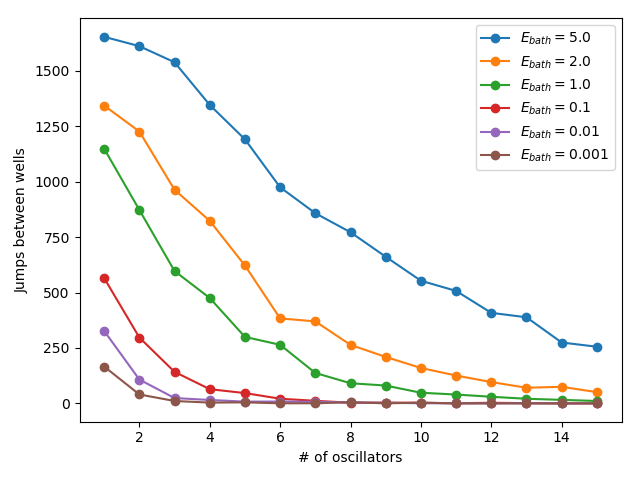
\includegraphics[width=0.7\textwidth]{Figures/change_E_number.png}
\caption{Number of jumps between the wells as a function of the number of oscillators in the heat bath for different values for the initial energy of the heat bath $E_{bath}$.
}
\label{fig:changing_E}
\end{figure} 

In Figure (\ref{fig:changing_E}) we can evidence that the different initial energies of the heat bath will result in a change of scale of the number of jumps that the particle suffers. The overall behavior of dissipation is continued to be present. For a heat bath with a high initial energy or \say{temperature} we see that the particle jumps between the wells more times than for a small energy but when the number of oscillators increases then the jumps decrease. When we \say{freeze} the heat bath by giving it a low initial energy we experience less jumps between the wells and a faster decay of it when the number of oscillators increase. Then we can conclude that the overall consequence of changing the initial energy of the heat bath will be a scaling factor in the exponential decay of the jumps.



\subsubsection{Changing the height of the potential barrier}
The particle of the central system is located on the unstable equilibrium unless otherwise stated for the simulations done in this work, then a very interesting parameter to study is the difference in the dynamics when the height of the potential barrier where the unstable equilibrium point is changed. We recall that the shape of the quartic potential for the particle is given by equation (\ref{eq:potential}) where the parameters $a$ and $b$ are in charge of the shape of the double well potential.\par 
\begin{figure}[H]
\centering
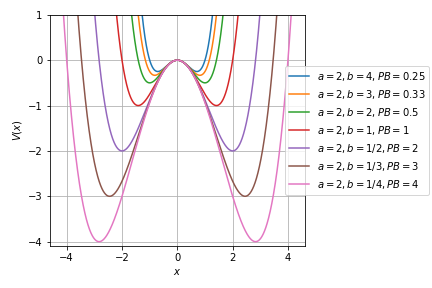
\includegraphics[width=0.7\textwidth]{Figures/double_well_PB_scale.png}
\caption{Shape of the double well potential keeping the same value of $a$ but changing the value of $b$.
}
\label{fig:PB_scale}
\end{figure} 

We have shown previously in equation (\ref{eq:PB_eq}) that the height of the potential barrier is completely determined by the parameters $a$ and $b$ and that the resonance frequency of small oscillations for the two minima is given by equation (\ref{eq:freq_small_oscillations}) which only depends on parameter $a$. This ideas are relevant to determine how to change the potential barrier height, in general there will be two ways in which we can change this height. If we change only $b$ we will rescale the whole potential, this means that the resonance frequency will change and the particle will have to travel more distance in general to go from one well to the other. The difference between changing the height this way is shown in Figure (\ref{fig:PB_scale}) where the shape of the potential is completely scaled.\par 

\begin{figure}[H]
\centering
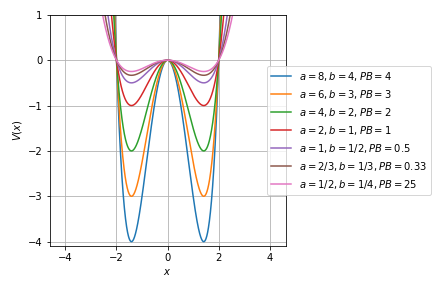
\includegraphics[width=0.7\textwidth]{Figures/double_well_PB.png}
\caption{Shape of the double well potential changing the values of $a$ and $b$ but keeping the ratio $a/b=2$.
}
\label{fig:PB_ratio}
\end{figure} 

The other way to change the height of the potential barrier is by changing both $a$ and $b$ but mantaining the ratio $a/b$, this ensures the roots of $V(x)$ to remain unchanged but makes the minimums of the potential deeper and as a consequence changing the height of the potential barrier as it is shown on Figure (\ref{fig:PB_ratio}). It is to be noted that this change of the wells' depth will in fact change the frequency of small oscillations  around the potential minima.

\begin{figure}[H]%
    \centering
    \subfloat[Changing only $b$]{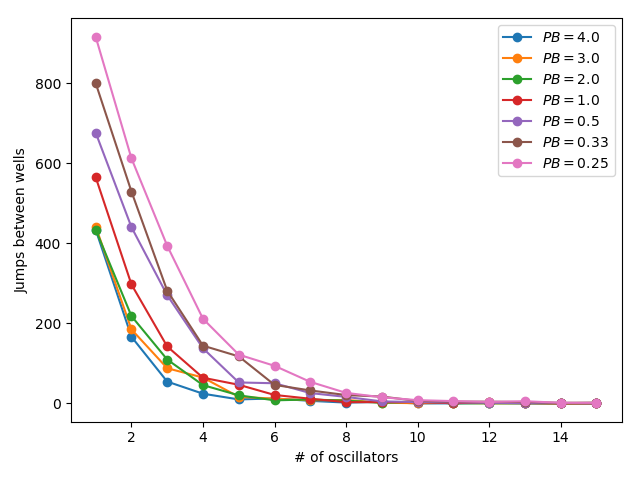
\includegraphics[width=10cm]{Figures/change_PB_a_quieto_number.png} }%
    \qquad
    \subfloat[Changing $a$ and $b$ but keeping the ratio $a/b=2$]{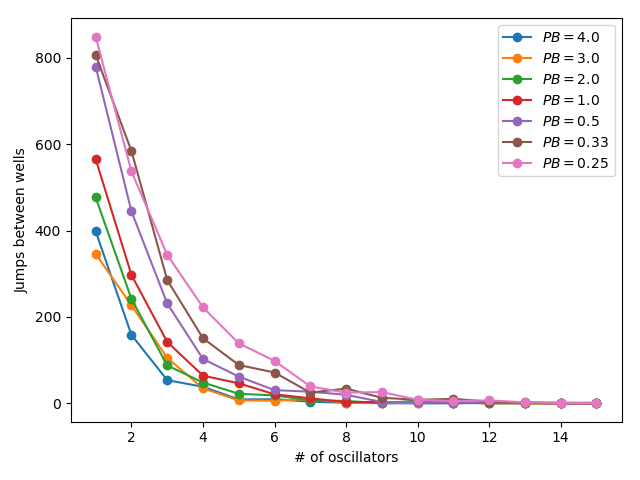
\includegraphics[width=10cm]{Figures/change_PB_a_b_number.png} }%
    \caption{Number of jumps between the wells as a function of the number of oscillators in the heat bath for different values for the height of the potential barrier $PB$}%
    \label{fig:changing_PB}%
\end{figure}

The height of the potential barrier is an important parameter for the reason that whenever the particle is inside one of the wells it will need an energy near to the height of the potential barrier in order to be able to jump to the other side. If the potential barrier is small then the particle does not need a lot of energy to be given from the oscillators in order to be able to surpass it, while if the potential barrier is big then it will need the oscillators to synchronize in a way to be able to give the particle enough energy to jump to the other well. In Figure (\ref{fig:changing_PB}) we test both cases of changing the height of the potential barrier. The results coincide with the intuition in the sense of more height means less jumps and less height means more jumps, also when the bath is composed of more harmonic oscillators then the number of jumps reduce significantly. In Figure (\ref{fig:changing_PB}) we also evidence that there is not a significant difference on how we decide to change the height of the potential barrier as both cases have similar results on the counts of jumps.






